\chapter{基本模型计算机设计实验}

\section{实验内容}

设计 8 位 CISC 模型计算机。

\begin{enumerate}
    
    \item 深入理解基本模型计算机的功能、组成知识;

    \item 深入学习计算机各类典型指令的执行流程;

    \item 学习微程序控制器的设计过程和相关技术,掌握 LPM\_ROM 的配置方法;

    \item 在掌握部件单元电路实验的基础上,进一步将单元电路组成系统,构造一台基本模型计算机;

    \item 定义五条机器指令,并编写相应的微程序,上机调试,掌握计算机整机概念;
    
    \item 掌握微程序的设计方法,学会编写二进制微指令代码表;

    \item 通过熟悉较完整的计算机的设计,全面了解并掌握微程序控制方式计算机的设计方法。

\end{enumerate}

\section{实验原理}

在微过程的控制下自动产生各部件单元控制信号,实现特定的功能。试验中,计算机数据通路的控制将由微过程控制器来完成,CPU从内存中取出一条机器指令对应一个微程序。本实验采用五条机器指令:IN(输入),ADD(二进制加法),STA(存数据),OUT(输出),JMP(无条件跳转)。步骤如下:先根据pc的值读取内存中指定的指令(操作码,操作数的地址,操作结果的存储地址,下一条指令的地址)放入寄存器中,数据的前几位是操作码,也就是 CPU 的指令码,将该指令码送往 ALU(运算器),在解析出指令中的操作数等信息,对相应的数据进行相应的操作,完成特定的功能。微指令(微程序控制的计算机中,将由同时发出的控制信号所执行的一组微操作)。微操作码字段,又称操作控制字段,该字段指出微指令执行的微操作;微地址码字段,又称顺序控制字段,指出下一条要执行的微指令的地址。

\begin{figure}[H]
\centering
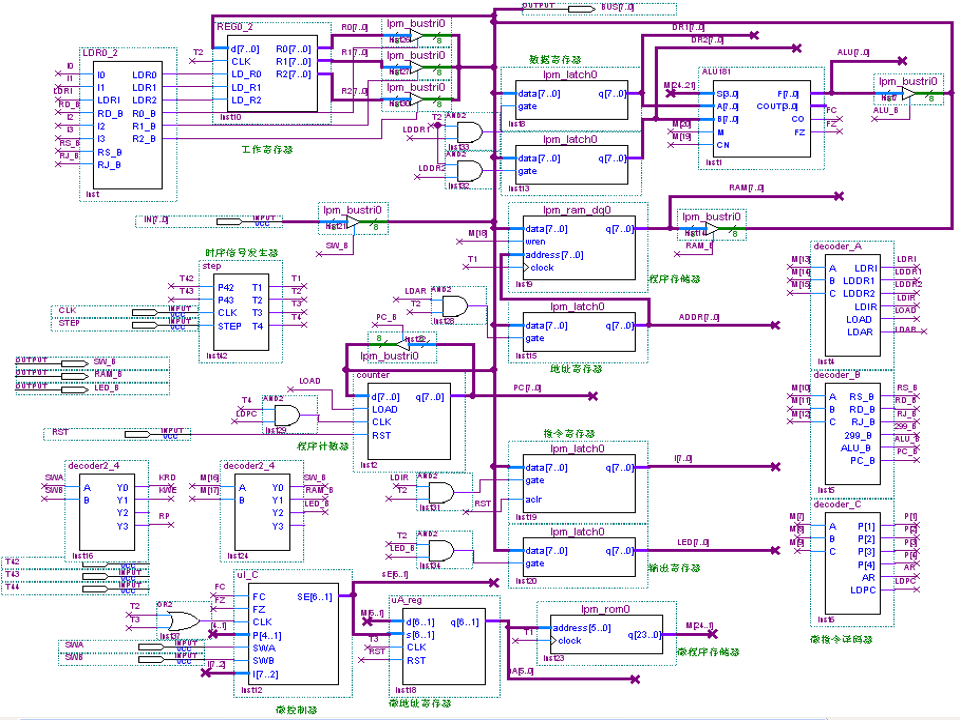
\includegraphics[width=\textwidth]{images/prin6_1.png}
\caption{基本模型计算机 CPU 顶层设计 原理图}
\label{fig:prin6_1}
\end{figure}

\begin{figure}[H]
\centering
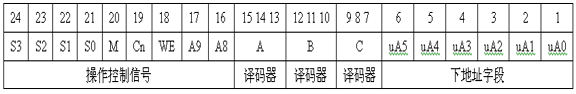
\includegraphics[width=\textwidth]{images/prin6_2.png}
\caption{微指令指令格式}
\label{fig:prin6_2}
\end{figure}

\begin{figure}[H]
\centering
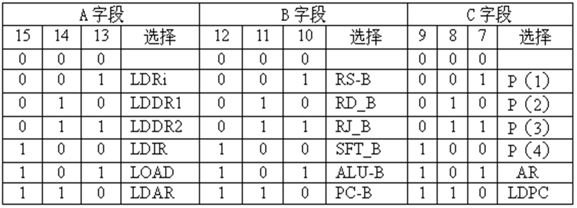
\includegraphics[width=\textwidth]{images/prin6_3.png}
\caption{微指令指令格式:图 \ref{fig:prin6_2} 中 A, B, C 字段详情}
\label{fig:prin6_3}
\end{figure}

\begin{figure}[H]
\centering
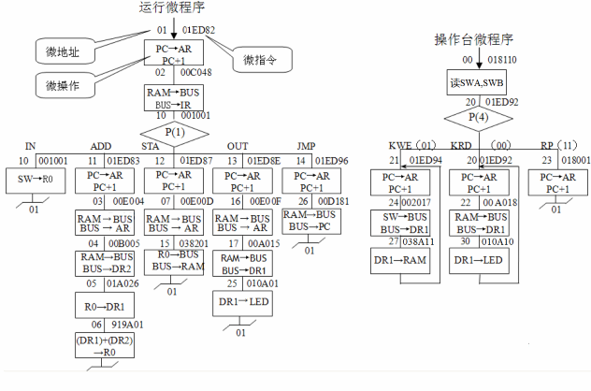
\includegraphics[width=\textwidth]{images/prin6_4.png}
\caption{微指令流程图}
\label{fig:prin6_4}
\end{figure}

\section{实验任务与实验步骤}

\begin{enumerate}
    \item 用图形编辑工具设计模型CPU的顶层电路原理图。
    \item 根据微程序的微操作,对于所需的控制信号,确定微指令,并确定微地址。
    \item 微程序流程图按微指令格式转化为“二进制微代码表”。
    \item 设计控制存储器LPM\_ROM。
    \item 对模型CPU的整机硬件电路进行编译、波形仿真和调试。
    \item 根据仿真波形,查找故障原因,排除故障,重新编译。
    \item 将编译通过的电路和应用程序下载到实验台上的FPGA中,在实验台上单步跟踪微程序的执行过程。
    \item 最终完成模型CPU的硬件电路设计和应用程序及微程序的设计和调试。 
\end{enumerate}


\section{实验结果分析}

\subsection{实验电路图}

根据原理图 \ref{fig:prin6_1} 绘制实验电路图 \ref{fig:bdf6}。

\begin{figure}[H]
\centering
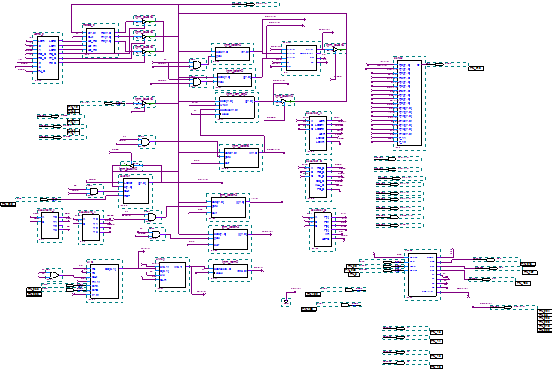
\includegraphics[width=\textwidth]{images/bdf6.png}
\caption{基本模型计算机实验 电路图}
\label{fig:bdf6}
\end{figure}

\subsection{储存器快照}

利用内存编辑器查看 ROM, RAM 快照 \ref{fig:mem6}。

\begin{figure}[H]
\centering
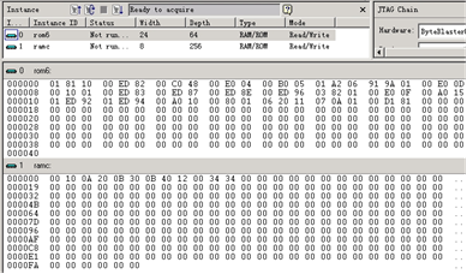
\includegraphics[width=\textwidth]{images/mem6.png}
\caption{基本模型计算机实验 ROM RAM 快照}
\label{fig:mem6}
\end{figure}

\subsection{仿真波形图}

利用 Quartus II 产生仿真波形图 \ref{fig:wave6}。

\begin{figure}[H]
\centering
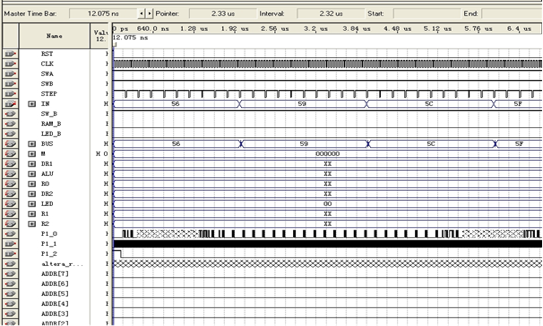
\includegraphics[width=\textwidth]{images/wave6.png}
\caption{基本模型计算机实验 仿真波形图}
\label{fig:wave6}
\end{figure}

\subsection{思考题}

\begin{enumerate}
    \item 除了已有的IN,ADD,STA,OUT,JMP指令外,再设计减法SUB,带进位加法ADC,逻辑与AND,逻辑或OR和 异或XOR指令,共10条指令,编写相应微程序流程图,写出微指令代码表。\footnote{从我能获取的参考资料上已不能找到完整的题目,参考他人的报告得到完整题目,如有错误,请指出。}
    
    \textbf{答}:
    
    \begin{figure}[H]
    \centering
    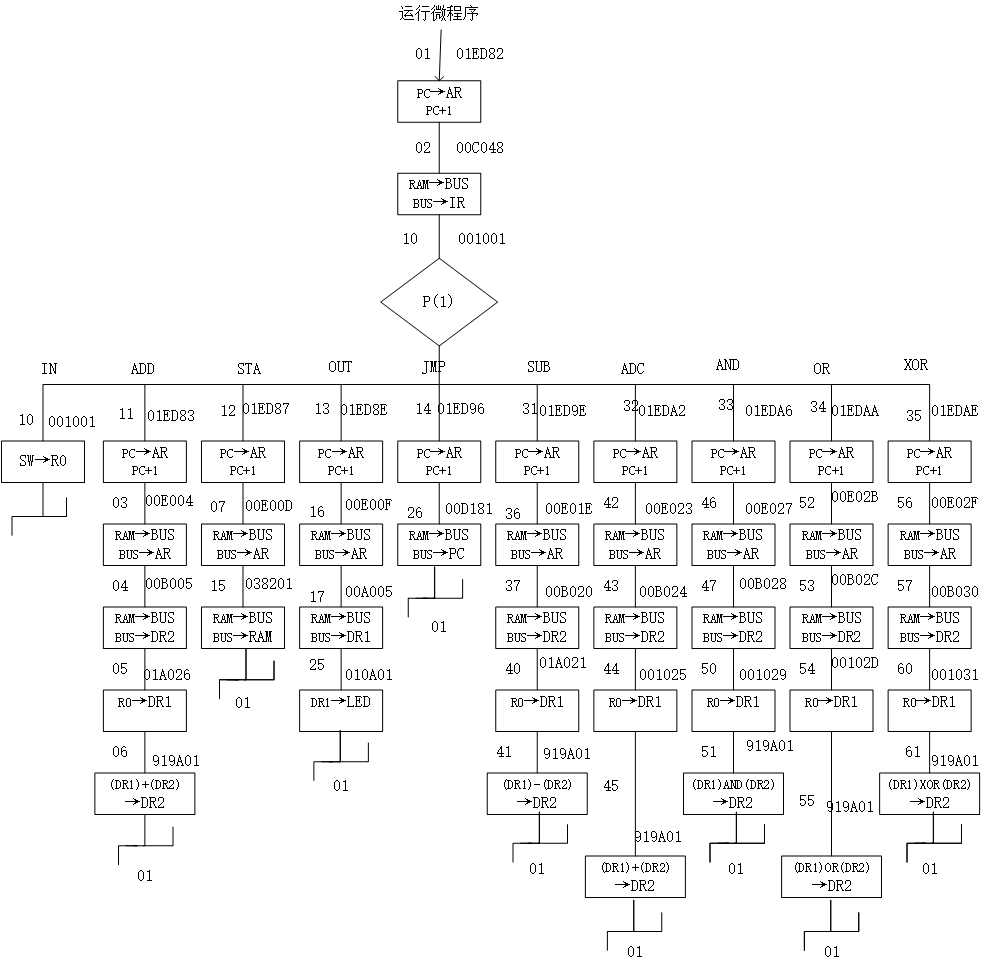
\includegraphics[width=\textwidth]{images/ans6_1.png}
    \caption{思考题答案 微程序流程图}
    \label{fig:ans6_1}
    \end{figure}
    
    微指令代码表如下:
    
    \begin{table}[H]
        \centering
        \begin{tabular}{|c|c|c|}
            \hline
            微地址 (OCT) & 助记符 & 微指令 (HEX) \\
            \hline
            10 & IN & 001001 \\
            \hline
            11 & ADD & 01ED83 \\
            \hline
            12 & STA & 01ED87 \\
            \hline
            13 & OUT & 01ED8E \\
            \hline
            14 & JMP & 01ED96 \\
            \hline
            31 & SUB & 01ED9E \\
            \hline
            31 & ADC & 01EDA2 \\
            \hline
            33 & AND & 01EDA6 \\
            \hline
            34 & OR & 01EDAA \\
            \hline
            35 & XOR & 01EDAE \\
            \hline
        \end{tabular}
        \caption{思考题答案 微指令代码表}
        \label{tab:ans6_1}
    \end{table}
    
\end{enumerate}
